\documentclass[1p]{elsarticle_modified}
%\bibliographystyle{elsarticle-num}

%\usepackage[colorlinks]{hyperref}
%\usepackage{abbrmath_seonhwa} %\Abb, \Ascr, \Acal ,\Abf, \Afrak
\usepackage{amsfonts}
\usepackage{amssymb}
\usepackage{amsmath}
\usepackage{amsthm}
\usepackage{scalefnt}
\usepackage{amsbsy}
\usepackage{kotex}
\usepackage{caption}
\usepackage{subfig}
\usepackage{color}
\usepackage{graphicx}
\usepackage{xcolor} %% white, black, red, green, blue, cyan, magenta, yellow
\usepackage{float}
\usepackage{setspace}
\usepackage{hyperref}

\usepackage{tikz}
\usetikzlibrary{arrows}

\usepackage{multirow}
\usepackage{array} % fixed length table
\usepackage{hhline}

%%%%%%%%%%%%%%%%%%%%%
\makeatletter
\renewcommand*\env@matrix[1][\arraystretch]{%
	\edef\arraystretch{#1}%
	\hskip -\arraycolsep
	\let\@ifnextchar\new@ifnextchar
	\array{*\c@MaxMatrixCols c}}
\makeatother %https://tex.stackexchange.com/questions/14071/how-can-i-increase-the-line-spacing-in-a-matrix
%%%%%%%%%%%%%%%

\usepackage[normalem]{ulem}

\newcommand{\msout}[1]{\ifmmode\text{\sout{\ensuremath{#1}}}\else\sout{#1}\fi}
%SOURCE: \msout is \stkout macro in https://tex.stackexchange.com/questions/20609/strikeout-in-math-mode

\newcommand{\cancel}[1]{
	\ifmmode
	{\color{red}\msout{#1}}
	\else
	{\color{red}\sout{#1}}
	\fi
}

\newcommand{\add}[1]{
	{\color{blue}\uwave{#1}}
}

\newcommand{\replace}[2]{
	\ifmmode
	{\color{red}\msout{#1}}{\color{blue}\uwave{#2}}
	\else
	{\color{red}\sout{#1}}{\color{blue}\uwave{#2}}
	\fi
}

\newcommand{\Sol}{\mathcal{S}} %segment
\newcommand{\D}{D} %diagram
\newcommand{\A}{\mathcal{A}} %arc


%%%%%%%%%%%%%%%%%%%%%%%%%%%%%5 test

\def\sl{\operatorname{\textup{SL}}(2,\Cbb)}
\def\psl{\operatorname{\textup{PSL}}(2,\Cbb)}
\def\quan{\mkern 1mu \triangleright \mkern 1mu}

\theoremstyle{definition}
\newtheorem{thm}{Theorem}[section]
\newtheorem{prop}[thm]{Proposition}
\newtheorem{lem}[thm]{Lemma}
\newtheorem{ques}[thm]{Question}
\newtheorem{cor}[thm]{Corollary}
\newtheorem{defn}[thm]{Definition}
\newtheorem{exam}[thm]{Example}
\newtheorem{rmk}[thm]{Remark}
\newtheorem{alg}[thm]{Algorithm}

\newcommand{\I}{\sqrt{-1}}
\begin{document}

%\begin{frontmatter}
%
%\title{Boundary parabolic representations of knots up to 8 crossings}
%
%%% Group authors per affiliation:
%\author{Yunhi Cho} 
%\address{Department of Mathematics, University of Seoul, Seoul, Korea}
%\ead{yhcho@uos.ac.kr}
%
%
%\author{Seonhwa Kim} %\fnref{s_kim}}
%\address{Center for Geometry and Physics, Institute for Basic Science, Pohang, 37673, Korea}
%\ead{ryeona17@ibs.re.kr}
%
%\author{Hyuk Kim}
%\address{Department of Mathematical Sciences, Seoul National University, Seoul 08826, Korea}
%\ead{hyukkim@snu.ac.kr}
%
%\author{Seokbeom Yoon}
%\address{Department of Mathematical Sciences, Seoul National University, Seoul, 08826,  Korea}
%\ead{sbyoon15@snu.ac.kr}
%
%\begin{abstract}
%We find all boundary parabolic representation of knots up to 8 crossings.
%
%\end{abstract}
%\begin{keyword}
%    \MSC[2010] 57M25 
%\end{keyword}
%
%\end{frontmatter}

%\linenumbers
%\tableofcontents
%
\newcommand\colored[1]{\textcolor{white}{\rule[-0.35ex]{0.8em}{1.4ex}}\kern-0.8em\color{red} #1}%
%\newcommand\colored[1]{\textcolor{white}{ #1}\kern-2.17ex	\textcolor{white}{ #1}\kern-1.81ex	\textcolor{white}{ #1}\kern-2.15ex\color{red}#1	}

{\Large $\underline{11a_{329}~(K11a_{329})}$}

\setlength{\tabcolsep}{10pt}
\renewcommand{\arraystretch}{1.6}
\vspace{1cm}\begin{tabular}{m{100pt}>{\centering\arraybackslash}m{274pt}}
\multirow{5}{120pt}{
	\centering
	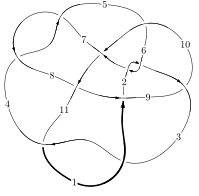
\includegraphics[width=112pt]{../../../GIT/diagram.site/Diagrams/png/578_11a_329.png}\\
\ \ \ A knot diagram\footnotemark}&
\allowdisplaybreaks
\textbf{Linearized knot diagam} \\
\cline{2-2}
 &
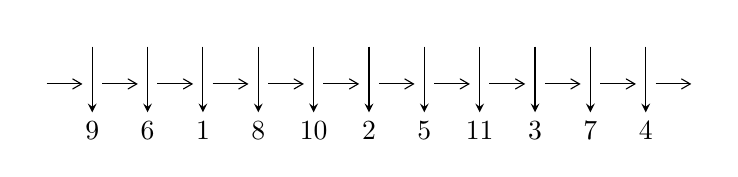
\begin{tikzpicture}[x=20pt, y=17pt]
	% nodes
	\node (C0) at (0, 0) {};
	\node (C1) at (1, 0) {};
	\node (C1U) at (1, +1) {};
	\node (C1D) at (1, -1) {9};

	\node (C2) at (2, 0) {};
	\node (C2U) at (2, +1) {};
	\node (C2D) at (2, -1) {6};

	\node (C3) at (3, 0) {};
	\node (C3U) at (3, +1) {};
	\node (C3D) at (3, -1) {1};

	\node (C4) at (4, 0) {};
	\node (C4U) at (4, +1) {};
	\node (C4D) at (4, -1) {8};

	\node (C5) at (5, 0) {};
	\node (C5U) at (5, +1) {};
	\node (C5D) at (5, -1) {10};

	\node (C6) at (6, 0) {};
	\node (C6U) at (6, +1) {};
	\node (C6D) at (6, -1) {2};

	\node (C7) at (7, 0) {};
	\node (C7U) at (7, +1) {};
	\node (C7D) at (7, -1) {5};

	\node (C8) at (8, 0) {};
	\node (C8U) at (8, +1) {};
	\node (C8D) at (8, -1) {11};

	\node (C9) at (9, 0) {};
	\node (C9U) at (9, +1) {};
	\node (C9D) at (9, -1) {3};

	\node (C10) at (10, 0) {};
	\node (C10U) at (10, +1) {};
	\node (C10D) at (10, -1) {7};

	\node (C11) at (11, 0) {};
	\node (C11U) at (11, +1) {};
	\node (C11D) at (11, -1) {4};
	\node (C12) at (12, 0) {};

	% arrows
	\draw[->,>={angle 60}]
	(C0) edge (C1) (C1) edge (C2) (C2) edge (C3) (C3) edge (C4) (C4) edge (C5) (C5) edge (C6) (C6) edge (C7) (C7) edge (C8) (C8) edge (C9) (C9) edge (C10) (C10) edge (C11) (C11) edge (C12) ;	\draw[->,>=stealth]
	(C1U) edge (C1D) (C2U) edge (C2D) (C3U) edge (C3D) (C4U) edge (C4D) (C5U) edge (C5D) (C6U) edge (C6D) (C7U) edge (C7D) (C8U) edge (C8D) (C9U) edge (C9D) (C10U) edge (C10D) (C11U) edge (C11D) ;
	\end{tikzpicture} \\
\hhline{~~} \\& 
\textbf{Solving Sequence} \\ \cline{2-2} 
 &
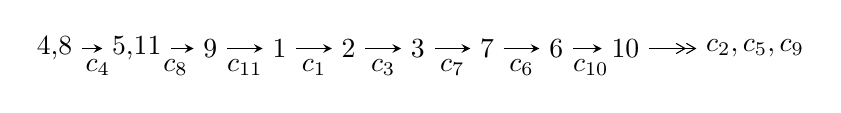
\begin{tikzpicture}[x=25pt, y=7pt]
	% node
	\node (A0) at (-1/8, 0) {4,8};
	\node (A1) at (17/16, 0) {5,11};
	\node (A2) at (17/8, 0) {9};
	\node (A3) at (25/8, 0) {1};
	\node (A4) at (33/8, 0) {2};
	\node (A5) at (41/8, 0) {3};
	\node (A6) at (49/8, 0) {7};
	\node (A7) at (57/8, 0) {6};
	\node (A8) at (65/8, 0) {10};
	\node (C1) at (1/2, -1) {$c_{4}$};
	\node (C2) at (13/8, -1) {$c_{8}$};
	\node (C3) at (21/8, -1) {$c_{11}$};
	\node (C4) at (29/8, -1) {$c_{1}$};
	\node (C5) at (37/8, -1) {$c_{3}$};
	\node (C6) at (45/8, -1) {$c_{7}$};
	\node (C7) at (53/8, -1) {$c_{6}$};
	\node (C8) at (61/8, -1) {$c_{10}$};
	\node (A9) at (10, 0) {$c_{2},c_{5},c_{9}$};

	% edge
	\draw[->,>=stealth]	
	(A0) edge (A1) (A1) edge (A2) (A2) edge (A3) (A3) edge (A4) (A4) edge (A5) (A5) edge (A6) (A6) edge (A7) (A7) edge (A8) ;
	\draw[->>,>={angle 60}]	
	(A8) edge (A9);
\end{tikzpicture} \\ 

\end{tabular} \\

\footnotetext{
The image of knot diagram is generated by the software ``\textbf{Draw programme}" developed by Andrew Bartholomew(\url{http://www.layer8.co.uk/maths/draw/index.htm\#Running-draw}), where we modified some parts for our purpose(\url{https://github.com/CATsTAILs/LinksPainter}).
}\phantom \\ \newline 
\centering \textbf{Ideals for irreducible components\footnotemark of $X_{\text{par}}$} 
 
\begin{align*}
I^u_{1}&=\langle 
b- u,\;7480949 u^{26}+102501940 u^{25}+\cdots+35850519 a+58313900,\;u^{27}+u^{26}+\cdots+4 u-1\rangle \\
I^u_{2}&=\langle 
-1.25488\times10^{119} u^{63}-5.93390\times10^{119} u^{62}+\cdots+1.36032\times10^{119} b-4.57609\times10^{119},\\
\phantom{I^u_{2}}&\phantom{= \langle  }-7.61826\times10^{119} u^{63}-3.45060\times10^{120} u^{62}+\cdots+4.08097\times10^{119} a+8.20476\times10^{119},\\
\phantom{I^u_{2}}&\phantom{= \langle  }u^{64}+5 u^{63}+\cdots+9 u+1\rangle \\
I^u_{3}&=\langle 
b+u,\;u^2+a+u,\;u^3+u-1\rangle \\
I^u_{4}&=\langle 
b+u,\;-2 u^7+u^6-7 u^5+u^4-10 u^3+a-7 u,\;u^8- u^7+4 u^6-2 u^5+6 u^4-2 u^3+5 u^2- u+1\rangle \\
I^u_{5}&=\langle 
u^6- u^5+3 u^4-7 u^3+6 u^2+2 b-10 u+5,\;-5 u^7-22 u^5+12 u^4-41 u^3+24 u^2+6 a-27 u+11,\\
\phantom{I^u_{5}}&\phantom{= \langle  }u^8+5 u^6-3 u^5+10 u^4-9 u^3+9 u^2-7 u+3\rangle \\
\\
\end{align*}
\raggedright * 5 irreducible components of $\dim_{\mathbb{C}}=0$, with total 110 representations.\\
\footnotetext{All coefficients of polynomials are rational numbers. But the coefficients are sometimes approximated in decimal forms when there is not enough margin.}
\newpage
\renewcommand{\arraystretch}{1}
\centering \section*{I. $I^u_{1}= \langle b- u,\;7.48\times10^{6} u^{26}+1.03\times10^{8} u^{25}+\cdots+3.59\times10^{7} a+5.83\times10^{7},\;u^{27}+u^{26}+\cdots+4 u-1 \rangle$}
\flushleft \textbf{(i) Arc colorings}\\
\begin{tabular}{m{7pt} m{180pt} m{7pt} m{180pt} }
\flushright $a_{4}=$&$\begin{pmatrix}1\\0\end{pmatrix}$ \\
\flushright $a_{8}=$&$\begin{pmatrix}0\\u\end{pmatrix}$ \\
\flushright $a_{5}=$&$\begin{pmatrix}1\\u^2\end{pmatrix}$ \\
\flushright $a_{11}=$&$\begin{pmatrix}-0.208671 u^{26}-2.85915 u^{25}+\cdots+7.44217 u-1.62658\\u\end{pmatrix}$ \\
\flushright $a_{9}=$&$\begin{pmatrix}-3.27801 u^{26}+5.32766 u^{25}+\cdots+46.4586 u-8.94242\\1.20999 u^{26}-3.00055 u^{25}+\cdots-9.39324 u+2.65048\end{pmatrix}$ \\
\flushright $a_{1}=$&$\begin{pmatrix}-0.208671 u^{26}-2.85915 u^{25}+\cdots+6.44217 u-1.62658\\u\end{pmatrix}$ \\
\flushright $a_{2}=$&$\begin{pmatrix}-2.58876 u^{26}-0.102742 u^{25}+\cdots-3.92105 u-2.07685\\0.977408 u^{26}+0.220438 u^{25}+\cdots-3.89929 u+0.517993\end{pmatrix}$ \\
\flushright $a_{3}=$&$\begin{pmatrix}2.65048 u^{26}+3.86047 u^{25}+\cdots+0.791902 u+1.20867\\- u^2\end{pmatrix}$ \\
\flushright $a_{7}=$&$\begin{pmatrix}u\\u^3+u\end{pmatrix}$ \\
\flushright $a_{6}=$&$\begin{pmatrix}3.03935 u^{26}+5.72431 u^{25}+\cdots+8.43055 u-4.17643\\-0.810224 u^{26}-2.02363 u^{25}+\cdots-2.57059 u+0.767074\end{pmatrix}$ \\
\flushright $a_{10}=$&$\begin{pmatrix}-0.606939 u^{26}-0.979932 u^{25}+\cdots+15.1011 u-3.18665\\0.175698 u^{26}-1.25035 u^{25}+\cdots-0.849262 u+0.717414\end{pmatrix}$\\ \flushright $a_{10}=$&$\begin{pmatrix}-0.606939 u^{26}-0.979932 u^{25}+\cdots+15.1011 u-3.18665\\0.175698 u^{26}-1.25035 u^{25}+\cdots-0.849262 u+0.717414\end{pmatrix}$\\&\end{tabular}
\flushleft \textbf{(ii) Obstruction class $= -1$}\\~\\
\flushleft \textbf{(iii) Cusp Shapes $= \frac{26113891}{3983391} u^{26}+\frac{16946267}{3983391} u^{25}+\cdots-\frac{13443049}{442599} u-\frac{51593591}{3983391}$}\\~\\
\newpage\renewcommand{\arraystretch}{1}
\flushleft \textbf{(iv) u-Polynomials at the component}\newline \\
\begin{tabular}{m{50pt}|m{274pt}}
Crossings & \hspace{64pt}u-Polynomials at each crossing \\
\hline $$\begin{aligned}c_{1},c_{10}\end{aligned}$$&$\begin{aligned}
&u^{27}-2 u^{26}+\cdots-10 u+3
\end{aligned}$\\
\hline $$\begin{aligned}c_{2},c_{6}\end{aligned}$$&$\begin{aligned}
&u^{27}+8 u^{26}+\cdots+110 u+12
\end{aligned}$\\
\hline $$\begin{aligned}c_{3},c_{4},c_{7}\\c_{11}\end{aligned}$$&$\begin{aligned}
&u^{27}- u^{26}+\cdots+4 u+1
\end{aligned}$\\
\hline $$\begin{aligned}c_{5},c_{9}\end{aligned}$$&$\begin{aligned}
&u^{27}+12 u^{25}+\cdots+15 u^2+1
\end{aligned}$\\
\hline $$\begin{aligned}c_{8}\end{aligned}$$&$\begin{aligned}
&u^{27}-20 u^{26}+\cdots-1284 u+180
\end{aligned}$\\
\hline
\end{tabular}\\~\\
\newpage\renewcommand{\arraystretch}{1}
\flushleft \textbf{(v) Riley Polynomials at the component}\newline \\
\begin{tabular}{m{50pt}|m{274pt}}
Crossings & \hspace{64pt}Riley Polynomials at each crossing \\
\hline $$\begin{aligned}c_{1},c_{10}\end{aligned}$$&$\begin{aligned}
&y^{27}+4 y^{26}+\cdots+4 y-9
\end{aligned}$\\
\hline $$\begin{aligned}c_{2},c_{6}\end{aligned}$$&$\begin{aligned}
&y^{27}+14 y^{26}+\cdots+700 y-144
\end{aligned}$\\
\hline $$\begin{aligned}c_{3},c_{4},c_{7}\\c_{11}\end{aligned}$$&$\begin{aligned}
&y^{27}+27 y^{26}+\cdots-4 y-1
\end{aligned}$\\
\hline $$\begin{aligned}c_{5},c_{9}\end{aligned}$$&$\begin{aligned}
&y^{27}+24 y^{26}+\cdots-30 y-1
\end{aligned}$\\
\hline $$\begin{aligned}c_{8}\end{aligned}$$&$\begin{aligned}
&y^{27}-2 y^{26}+\cdots+561816 y-32400
\end{aligned}$\\
\hline
\end{tabular}\\~\\
\newpage\flushleft \textbf{(vi) Complex Volumes and Cusp Shapes}
$$\begin{array}{c|c|c}  
\text{Solutions to }I^u_{1}& \I (\text{vol} + \sqrt{-1}CS) & \text{Cusp shape}\\
 \hline 
\begin{aligned}
u &= -0.886580 + 0.019207 I \\
a &= -1.057340 + 0.497197 I \\
b &= -0.886580 + 0.019207 I\end{aligned}
 & \phantom{-}0.96030 + 6.99778 I & -11.49841 - 6.31594 I \\ \hline\begin{aligned}
u &= -0.886580 - 0.019207 I \\
a &= -1.057340 - 0.497197 I \\
b &= -0.886580 - 0.019207 I\end{aligned}
 & \phantom{-}0.96030 - 6.99778 I & -11.49841 + 6.31594 I \\ \hline\begin{aligned}
u &= -0.236028 + 1.095620 I \\
a &= -0.798201 + 0.061958 I \\
b &= -0.236028 + 1.095620 I\end{aligned}
 & \phantom{-}4.10301 - 1.11169 I & -6.68347 + 2.36909 I \\ \hline\begin{aligned}
u &= -0.236028 - 1.095620 I \\
a &= -0.798201 - 0.061958 I \\
b &= -0.236028 - 1.095620 I\end{aligned}
 & \phantom{-}4.10301 + 1.11169 I & -6.68347 - 2.36909 I \\ \hline\begin{aligned}
u &= \phantom{-}0.868007 + 0.115359 I \\
a &= \phantom{-}0.768649 - 0.417549 I \\
b &= \phantom{-}0.868007 + 0.115359 I\end{aligned}
 & -2.19193 + 1.02446 I & -11.23776 - 6.18138 I \\ \hline\begin{aligned}
u &= \phantom{-}0.868007 - 0.115359 I \\
a &= \phantom{-}0.768649 + 0.417549 I \\
b &= \phantom{-}0.868007 - 0.115359 I\end{aligned}
 & -2.19193 - 1.02446 I & -11.23776 + 6.18138 I \\ \hline\begin{aligned}
u &= -0.003006 + 1.229040 I \\
a &= \phantom{-}1.65700 - 1.48184 I \\
b &= -0.003006 + 1.229040 I\end{aligned}
 & \phantom{-}9.55943 + 6.00813 I & -1.22265 - 6.13894 I \\ \hline\begin{aligned}
u &= -0.003006 - 1.229040 I \\
a &= \phantom{-}1.65700 + 1.48184 I \\
b &= -0.003006 - 1.229040 I\end{aligned}
 & \phantom{-}9.55943 - 6.00813 I & -1.22265 + 6.13894 I \\ \hline\begin{aligned}
u &= -0.045846 + 1.255570 I \\
a &= -1.24858 - 0.95153 I \\
b &= -0.045846 + 1.255570 I\end{aligned}
 & \phantom{-}6.76407 - 1.62647 I & -5.58254 + 2.60825 I \\ \hline\begin{aligned}
u &= -0.045846 - 1.255570 I \\
a &= -1.24858 + 0.95153 I \\
b &= -0.045846 - 1.255570 I\end{aligned}
 & \phantom{-}6.76407 + 1.62647 I & -5.58254 - 2.60825 I\\
 \hline 
 \end{array}$$\newpage$$\begin{array}{c|c|c}  
\text{Solutions to }I^u_{1}& \I (\text{vol} + \sqrt{-1}CS) & \text{Cusp shape}\\
 \hline 
\begin{aligned}
u &= -0.029913 + 1.343500 I \\
a &= \phantom{-}0.37553 - 1.49753 I \\
b &= -0.029913 + 1.343500 I\end{aligned}
 & \phantom{-}9.97119 - 1.49427 I & \phantom{-}0.080207 + 0.920031 I \\ \hline\begin{aligned}
u &= -0.029913 - 1.343500 I \\
a &= \phantom{-}0.37553 + 1.49753 I \\
b &= -0.029913 - 1.343500 I\end{aligned}
 & \phantom{-}9.97119 + 1.49427 I & \phantom{-}0.080207 - 0.920031 I \\ \hline\begin{aligned}
u &= \phantom{-}0.524847 + 1.241400 I \\
a &= \phantom{-}0.633730 - 0.220695 I \\
b &= \phantom{-}0.524847 + 1.241400 I\end{aligned}
 & \phantom{-}2.50522 - 4.33326 I & -7.76207 - 3.39042 I \\ \hline\begin{aligned}
u &= \phantom{-}0.524847 - 1.241400 I \\
a &= \phantom{-}0.633730 + 0.220695 I \\
b &= \phantom{-}0.524847 - 1.241400 I\end{aligned}
 & \phantom{-}2.50522 + 4.33326 I & -7.76207 + 3.39042 I \\ \hline\begin{aligned}
u &= -0.580317 + 0.090563 I \\
a &= -0.597417 + 1.252030 I \\
b &= -0.580317 + 0.090563 I\end{aligned}
 & \phantom{-}3.08469 - 2.64958 I & -9.08747 + 2.09938 I \\ \hline\begin{aligned}
u &= -0.580317 - 0.090563 I \\
a &= -0.597417 - 1.252030 I \\
b &= -0.580317 - 0.090563 I\end{aligned}
 & \phantom{-}3.08469 + 2.64958 I & -9.08747 - 2.09938 I \\ \hline\begin{aligned}
u &= \phantom{-}0.10388 + 1.45531 I \\
a &= \phantom{-}0.370550 - 0.378802 I \\
b &= \phantom{-}0.10388 + 1.45531 I\end{aligned}
 & \phantom{-}10.25310 - 0.47528 I & -1.44372 + 0. I\phantom{ +0.000000I} \\ \hline\begin{aligned}
u &= \phantom{-}0.10388 - 1.45531 I \\
a &= \phantom{-}0.370550 + 0.378802 I \\
b &= \phantom{-}0.10388 - 1.45531 I\end{aligned}
 & \phantom{-}10.25310 + 0.47528 I & -1.44372 + 0. I\phantom{ +0.000000I} \\ \hline\begin{aligned}
u &= -0.45771 + 1.48529 I \\
a &= -0.908211 - 0.286969 I \\
b &= -0.45771 + 1.48529 I\end{aligned}
 & \phantom{-}12.64960 + 6.10710 I & -1.83403 - 3.86721 I \\ \hline\begin{aligned}
u &= -0.45771 - 1.48529 I \\
a &= -0.908211 + 0.286969 I \\
b &= -0.45771 - 1.48529 I\end{aligned}
 & \phantom{-}12.64960 - 6.10710 I & -1.83403 + 3.86721 I\\
 \hline 
 \end{array}$$\newpage$$\begin{array}{c|c|c}  
\text{Solutions to }I^u_{1}& \I (\text{vol} + \sqrt{-1}CS) & \text{Cusp shape}\\
 \hline 
\begin{aligned}
u &= -0.47966 + 1.48279 I \\
a &= -1.135590 - 0.392236 I \\
b &= -0.47966 + 1.48279 I\end{aligned}
 & \phantom{-}10.7046 + 17.4305 I & -4.97020 - 8.80041 I \\ \hline\begin{aligned}
u &= -0.47966 - 1.48279 I \\
a &= -1.135590 + 0.392236 I \\
b &= -0.47966 - 1.48279 I\end{aligned}
 & \phantom{-}10.7046 - 17.4305 I & -4.97020 + 8.80041 I \\ \hline\begin{aligned}
u &= \phantom{-}0.47037 + 1.48644 I \\
a &= \phantom{-}1.021560 - 0.423137 I \\
b &= \phantom{-}0.47037 + 1.48644 I\end{aligned}
 & \phantom{-}7.11389 - 11.36350 I & -6.87134 + 6.73077 I \\ \hline\begin{aligned}
u &= \phantom{-}0.47037 - 1.48644 I \\
a &= \phantom{-}1.021560 + 0.423137 I \\
b &= \phantom{-}0.47037 - 1.48644 I\end{aligned}
 & \phantom{-}7.11389 + 11.36350 I & -6.87134 - 6.73077 I \\ \hline\begin{aligned}
u &= \phantom{-}0.275286\phantom{ +0.000000I} \\
a &= -0.867193\phantom{ +0.000000I} \\
b &= \phantom{-}0.275286\phantom{ +0.000000I}\end{aligned}
 & -0.622366\phantom{ +0.000000I} & -16.1230\phantom{ +0.000000I} \\ \hline\begin{aligned}
u &= \phantom{-}0.114320 + 0.213263 I \\
a &= -1.14807 + 5.10834 I \\
b &= \phantom{-}0.114320 + 0.213263 I\end{aligned}
 & -1.14394 + 1.30778 I & -18.3250 - 4.6536 I \\ \hline\begin{aligned}
u &= \phantom{-}0.114320 - 0.213263 I \\
a &= -1.14807 - 5.10834 I \\
b &= \phantom{-}0.114320 - 0.213263 I\end{aligned}
 & -1.14394 - 1.30778 I & -18.3250 + 4.6536 I\\
 \hline 
 \end{array}$$\newpage\newpage\renewcommand{\arraystretch}{1}
\centering \section*{II. $I^u_{2}= \langle -1.25\times10^{119} u^{63}-5.93\times10^{119} u^{62}+\cdots+1.36\times10^{119} b-4.58\times10^{119},\;-7.62\times10^{119} u^{63}-3.45\times10^{120} u^{62}+\cdots+4.08\times10^{119} a+8.20\times10^{119},\;u^{64}+5 u^{63}+\cdots+9 u+1 \rangle$}
\flushleft \textbf{(i) Arc colorings}\\
\begin{tabular}{m{7pt} m{180pt} m{7pt} m{180pt} }
\flushright $a_{4}=$&$\begin{pmatrix}1\\0\end{pmatrix}$ \\
\flushright $a_{8}=$&$\begin{pmatrix}0\\u\end{pmatrix}$ \\
\flushright $a_{5}=$&$\begin{pmatrix}1\\u^2\end{pmatrix}$ \\
\flushright $a_{11}=$&$\begin{pmatrix}1.86678 u^{63}+8.45535 u^{62}+\cdots+13.0919 u-2.01050\\0.922490 u^{63}+4.36213 u^{62}+\cdots+19.0193 u+3.36397\end{pmatrix}$ \\
\flushright $a_{9}=$&$\begin{pmatrix}-2.07092 u^{63}-9.95817 u^{62}+\cdots-51.5217 u-6.64500\\-0.765928 u^{63}-3.73638 u^{62}+\cdots-20.4529 u-4.25401\end{pmatrix}$ \\
\flushright $a_{1}=$&$\begin{pmatrix}0.944287 u^{63}+4.09322 u^{62}+\cdots-5.92732 u-5.37447\\0.922490 u^{63}+4.36213 u^{62}+\cdots+19.0193 u+3.36397\end{pmatrix}$ \\
\flushright $a_{2}=$&$\begin{pmatrix}-1.92058 u^{63}-9.65347 u^{62}+\cdots-55.0762 u-11.3256\\0.0555653 u^{63}+0.244446 u^{62}+\cdots+4.82412 u+0.229347\end{pmatrix}$ \\
\flushright $a_{3}=$&$\begin{pmatrix}5.08294 u^{63}+24.8391 u^{62}+\cdots+104.384 u+17.2019\\-0.828932 u^{63}-4.33500 u^{62}+\cdots-13.7757 u+0.631299\end{pmatrix}$ \\
\flushright $a_{7}=$&$\begin{pmatrix}u\\u^3+u\end{pmatrix}$ \\
\flushright $a_{6}=$&$\begin{pmatrix}-3.21107 u^{63}-15.6228 u^{62}+\cdots-65.7787 u-11.6119\\0.348757 u^{63}+1.59825 u^{62}+\cdots+16.3904 u+1.14200\end{pmatrix}$ \\
\flushright $a_{10}=$&$\begin{pmatrix}1.54638 u^{63}+7.15847 u^{62}+\cdots+9.16166 u-2.57721\\0.647718 u^{63}+2.94801 u^{62}+\cdots+12.6636 u+2.49217\end{pmatrix}$\\ \flushright $a_{10}=$&$\begin{pmatrix}1.54638 u^{63}+7.15847 u^{62}+\cdots+9.16166 u-2.57721\\0.647718 u^{63}+2.94801 u^{62}+\cdots+12.6636 u+2.49217\end{pmatrix}$\\&\end{tabular}
\flushleft \textbf{(ii) Obstruction class $= -1$}\\~\\
\flushleft \textbf{(iii) Cusp Shapes $= -1.07366 u^{63}-4.33095 u^{62}+\cdots+40.1271 u+1.41454$}\\~\\
\newpage\renewcommand{\arraystretch}{1}
\flushleft \textbf{(iv) u-Polynomials at the component}\newline \\
\begin{tabular}{m{50pt}|m{274pt}}
Crossings & \hspace{64pt}u-Polynomials at each crossing \\
\hline $$\begin{aligned}c_{1},c_{10}\end{aligned}$$&$\begin{aligned}
&u^{64}+2 u^{63}+\cdots-126 u+177
\end{aligned}$\\
\hline $$\begin{aligned}c_{2},c_{6}\end{aligned}$$&$\begin{aligned}
&(u^{32}-3 u^{31}+\cdots-10 u+3)^{2}
\end{aligned}$\\
\hline $$\begin{aligned}c_{3},c_{4},c_{7}\\c_{11}\end{aligned}$$&$\begin{aligned}
&u^{64}-5 u^{63}+\cdots-9 u+1
\end{aligned}$\\
\hline $$\begin{aligned}c_{5},c_{9}\end{aligned}$$&$\begin{aligned}
&u^{64}- u^{63}+\cdots-16935 u+15481
\end{aligned}$\\
\hline $$\begin{aligned}c_{8}\end{aligned}$$&$\begin{aligned}
&(u^{32}+10 u^{31}+\cdots+99 u+19)^{2}
\end{aligned}$\\
\hline
\end{tabular}\\~\\
\newpage\renewcommand{\arraystretch}{1}
\flushleft \textbf{(v) Riley Polynomials at the component}\newline \\
\begin{tabular}{m{50pt}|m{274pt}}
Crossings & \hspace{64pt}Riley Polynomials at each crossing \\
\hline $$\begin{aligned}c_{1},c_{10}\end{aligned}$$&$\begin{aligned}
&y^{64}+4 y^{63}+\cdots+305202 y+31329
\end{aligned}$\\
\hline $$\begin{aligned}c_{2},c_{6}\end{aligned}$$&$\begin{aligned}
&(y^{32}+21 y^{31}+\cdots+74 y+9)^{2}
\end{aligned}$\\
\hline $$\begin{aligned}c_{3},c_{4},c_{7}\\c_{11}\end{aligned}$$&$\begin{aligned}
&y^{64}+49 y^{63}+\cdots-3 y+1
\end{aligned}$\\
\hline $$\begin{aligned}c_{5},c_{9}\end{aligned}$$&$\begin{aligned}
&y^{64}+11 y^{63}+\cdots+3729627377 y+239661361
\end{aligned}$\\
\hline $$\begin{aligned}c_{8}\end{aligned}$$&$\begin{aligned}
&(y^{32}+18 y^{31}+\cdots+3461 y+361)^{2}
\end{aligned}$\\
\hline
\end{tabular}\\~\\
\newpage\flushleft \textbf{(vi) Complex Volumes and Cusp Shapes}
$$\begin{array}{c|c|c}  
\text{Solutions to }I^u_{2}& \I (\text{vol} + \sqrt{-1}CS) & \text{Cusp shape}\\
 \hline 
\begin{aligned}
u &= \phantom{-}0.920222 + 0.395412 I \\
a &= -0.129317 + 1.135090 I \\
b &= -0.151131 + 1.300520 I\end{aligned}
 & \phantom{-}3.42651 + 2.86570 I & -5.40728 - 4.03056 I \\ \hline\begin{aligned}
u &= \phantom{-}0.920222 - 0.395412 I \\
a &= -0.129317 - 1.135090 I \\
b &= -0.151131 - 1.300520 I\end{aligned}
 & \phantom{-}3.42651 - 2.86570 I & -5.40728 + 4.03056 I \\ \hline\begin{aligned}
u &= -0.063212 + 0.940817 I \\
a &= \phantom{-}0.717133 + 0.574436 I \\
b &= \phantom{-}0.804979 - 0.202940 I\end{aligned}
 & -0.168876 + 0.846731 I & -12.88022 - 0.77932 I \\ \hline\begin{aligned}
u &= -0.063212 - 0.940817 I \\
a &= \phantom{-}0.717133 - 0.574436 I \\
b &= \phantom{-}0.804979 + 0.202940 I\end{aligned}
 & -0.168876 - 0.846731 I & -12.88022 + 0.77932 I \\ \hline\begin{aligned}
u &= \phantom{-}0.294249 + 1.039510 I \\
a &= -1.105040 + 0.363187 I \\
b &= -0.685111 - 0.128372 I\end{aligned}
 & \phantom{-}1.25382 - 4.32436 I & \phantom{-0.000000 } 0 \\ \hline\begin{aligned}
u &= \phantom{-}0.294249 - 1.039510 I \\
a &= -1.105040 - 0.363187 I \\
b &= -0.685111 + 0.128372 I\end{aligned}
 & \phantom{-}1.25382 + 4.32436 I & \phantom{-0.000000 } 0 \\ \hline\begin{aligned}
u &= \phantom{-}0.804979 + 0.202940 I \\
a &= -0.872180 - 0.573156 I \\
b &= -0.063212 - 0.940817 I\end{aligned}
 & -0.168876 - 0.846731 I & -12.88022 + 0.77932 I \\ \hline\begin{aligned}
u &= \phantom{-}0.804979 - 0.202940 I \\
a &= -0.872180 + 0.573156 I \\
b &= -0.063212 + 0.940817 I\end{aligned}
 & -0.168876 + 0.846731 I & -12.88022 - 0.77932 I \\ \hline\begin{aligned}
u &= -0.271195 + 1.153980 I \\
a &= \phantom{-}1.63456 + 0.62464 I \\
b &= \phantom{-}0.336277 - 1.364760 I\end{aligned}
 & \phantom{-}4.73825 + 4.95632 I & \phantom{-0.000000 } 0 \\ \hline\begin{aligned}
u &= -0.271195 - 1.153980 I \\
a &= \phantom{-}1.63456 - 0.62464 I \\
b &= \phantom{-}0.336277 + 1.364760 I\end{aligned}
 & \phantom{-}4.73825 - 4.95632 I & \phantom{-0.000000 } 0\\
 \hline 
 \end{array}$$\newpage$$\begin{array}{c|c|c}  
\text{Solutions to }I^u_{2}& \I (\text{vol} + \sqrt{-1}CS) & \text{Cusp shape}\\
 \hline 
\begin{aligned}
u &= -0.053296 + 1.199700 I \\
a &= \phantom{-}0.715928 + 0.774703 I \\
b &= \phantom{-}0.42436 - 1.68610 I\end{aligned}
 & \phantom{-}5.82389 + 3.48280 I & \phantom{-0.000000 } 0 \\ \hline\begin{aligned}
u &= -0.053296 - 1.199700 I \\
a &= \phantom{-}0.715928 - 0.774703 I \\
b &= \phantom{-}0.42436 + 1.68610 I\end{aligned}
 & \phantom{-}5.82389 - 3.48280 I & \phantom{-0.000000 } 0 \\ \hline\begin{aligned}
u &= -0.087790 + 1.202470 I \\
a &= -0.397620 + 0.281730 I \\
b &= -1.04393 - 1.82190 I\end{aligned}
 & \phantom{-}8.11459 + 3.37630 I & \phantom{-0.000000 } 0 \\ \hline\begin{aligned}
u &= -0.087790 - 1.202470 I \\
a &= -0.397620 - 0.281730 I \\
b &= -1.04393 + 1.82190 I\end{aligned}
 & \phantom{-}8.11459 - 3.37630 I & \phantom{-0.000000 } 0 \\ \hline\begin{aligned}
u &= -0.612602 + 0.471856 I \\
a &= \phantom{-}0.025706 + 1.164300 I \\
b &= \phantom{-}0.232794 + 1.231510 I\end{aligned}
 & \phantom{-}2.52109 - 1.66996 I & -6.36037 - 2.48874 I \\ \hline\begin{aligned}
u &= -0.612602 - 0.471856 I \\
a &= \phantom{-}0.025706 - 1.164300 I \\
b &= \phantom{-}0.232794 - 1.231510 I\end{aligned}
 & \phantom{-}2.52109 + 1.66996 I & -6.36037 + 2.48874 I \\ \hline\begin{aligned}
u &= \phantom{-}0.452635 + 1.145970 I \\
a &= -1.69479 + 0.14216 I \\
b &= -0.297614 - 1.338770 I\end{aligned}
 & \phantom{-}5.87133 - 7.92548 I & \phantom{-0.000000 } 0 \\ \hline\begin{aligned}
u &= \phantom{-}0.452635 - 1.145970 I \\
a &= -1.69479 - 0.14216 I \\
b &= -0.297614 + 1.338770 I\end{aligned}
 & \phantom{-}5.87133 + 7.92548 I & \phantom{-0.000000 } 0 \\ \hline\begin{aligned}
u &= -0.201492 + 1.219100 I \\
a &= -0.686845 + 0.005818 I \\
b &= -1.382930 + 0.232456 I\end{aligned}
 & \phantom{-}6.90028 + 0.03721 I & \phantom{-0.000000 } 0 \\ \hline\begin{aligned}
u &= -0.201492 - 1.219100 I \\
a &= -0.686845 - 0.005818 I \\
b &= -1.382930 - 0.232456 I\end{aligned}
 & \phantom{-}6.90028 - 0.03721 I & \phantom{-0.000000 } 0\\
 \hline 
 \end{array}$$\newpage$$\begin{array}{c|c|c}  
\text{Solutions to }I^u_{2}& \I (\text{vol} + \sqrt{-1}CS) & \text{Cusp shape}\\
 \hline 
\begin{aligned}
u &= -1.197290 + 0.312647 I \\
a &= -0.707406 + 0.535648 I \\
b &= -0.398045 + 1.299040 I\end{aligned}
 & \phantom{-}5.08314 + 11.58170 I & \phantom{-0.000000 } 0 \\ \hline\begin{aligned}
u &= -1.197290 - 0.312647 I \\
a &= -0.707406 - 0.535648 I \\
b &= -0.398045 - 1.299040 I\end{aligned}
 & \phantom{-}5.08314 - 11.58170 I & \phantom{-0.000000 } 0 \\ \hline\begin{aligned}
u &= \phantom{-}0.232794 + 1.231510 I \\
a &= -0.633433 + 0.339154 I \\
b &= -0.612602 + 0.471856 I\end{aligned}
 & \phantom{-}2.52109 - 1.66996 I & \phantom{-0.000000 } 0 \\ \hline\begin{aligned}
u &= \phantom{-}0.232794 - 1.231510 I \\
a &= -0.633433 - 0.339154 I \\
b &= -0.612602 - 0.471856 I\end{aligned}
 & \phantom{-}2.52109 + 1.66996 I & \phantom{-0.000000 } 0 \\ \hline\begin{aligned}
u &= -0.339847 + 1.221780 I \\
a &= \phantom{-}0.956485 - 0.589998 I \\
b &= \phantom{-}0.120701 - 0.199374 I\end{aligned}
 & \phantom{-}6.38478 + 6.22988 I & \phantom{-0.000000 } 0 \\ \hline\begin{aligned}
u &= -0.339847 - 1.221780 I \\
a &= \phantom{-}0.956485 + 0.589998 I \\
b &= \phantom{-}0.120701 + 0.199374 I\end{aligned}
 & \phantom{-}6.38478 - 6.22988 I & \phantom{-0.000000 } 0 \\ \hline\begin{aligned}
u &= \phantom{-}0.276431 + 1.243720 I \\
a &= -0.639083 - 0.172102 I \\
b &= -0.230618 + 0.105542 I\end{aligned}
 & \phantom{-}2.72784 - 2.52152 I & \phantom{-0.000000 } 0 \\ \hline\begin{aligned}
u &= \phantom{-}0.276431 - 1.243720 I \\
a &= -0.639083 + 0.172102 I \\
b &= -0.230618 - 0.105542 I\end{aligned}
 & \phantom{-}2.72784 + 2.52152 I & \phantom{-0.000000 } 0 \\ \hline\begin{aligned}
u &= \phantom{-}0.397836 + 1.218830 I \\
a &= \phantom{-}0.644295 - 0.250433 I \\
b &= \phantom{-}1.211970 + 0.440132 I\end{aligned}
 & \phantom{-}1.24375 - 5.55297 I & \phantom{-0.000000 } 0 \\ \hline\begin{aligned}
u &= \phantom{-}0.397836 - 1.218830 I \\
a &= \phantom{-}0.644295 + 0.250433 I \\
b &= \phantom{-}1.211970 - 0.440132 I\end{aligned}
 & \phantom{-}1.24375 + 5.55297 I & \phantom{-0.000000 } 0\\
 \hline 
 \end{array}$$\newpage$$\begin{array}{c|c|c}  
\text{Solutions to }I^u_{2}& \I (\text{vol} + \sqrt{-1}CS) & \text{Cusp shape}\\
 \hline 
\begin{aligned}
u &= \phantom{-}1.211970 + 0.440132 I \\
a &= \phantom{-}0.590869 + 0.351158 I \\
b &= \phantom{-}0.397836 + 1.218830 I\end{aligned}
 & \phantom{-}1.24375 - 5.55297 I & \phantom{-0.000000 } 0 \\ \hline\begin{aligned}
u &= \phantom{-}1.211970 - 0.440132 I \\
a &= \phantom{-}0.590869 - 0.351158 I \\
b &= \phantom{-}0.397836 - 1.218830 I\end{aligned}
 & \phantom{-}1.24375 + 5.55297 I & \phantom{-0.000000 } 0 \\ \hline\begin{aligned}
u &= -0.685111 + 0.128372 I \\
a &= \phantom{-}1.26615 - 1.28343 I \\
b &= \phantom{-}0.294249 - 1.039510 I\end{aligned}
 & \phantom{-}1.25382 + 4.32436 I & -10.17044 - 8.05596 I \\ \hline\begin{aligned}
u &= -0.685111 - 0.128372 I \\
a &= \phantom{-}1.26615 + 1.28343 I \\
b &= \phantom{-}0.294249 + 1.039510 I\end{aligned}
 & \phantom{-}1.25382 - 4.32436 I & -10.17044 + 8.05596 I \\ \hline\begin{aligned}
u &= -0.151131 + 1.300520 I \\
a &= \phantom{-}0.803730 + 0.343215 I \\
b &= \phantom{-}0.920222 + 0.395412 I\end{aligned}
 & \phantom{-}3.42651 + 2.86570 I & \phantom{-0.000000 } 0 \\ \hline\begin{aligned}
u &= -0.151131 - 1.300520 I \\
a &= \phantom{-}0.803730 - 0.343215 I \\
b &= \phantom{-}0.920222 - 0.395412 I\end{aligned}
 & \phantom{-}3.42651 - 2.86570 I & \phantom{-0.000000 } 0 \\ \hline\begin{aligned}
u &= \phantom{-}0.090336 + 1.330560 I \\
a &= -0.986962 + 0.344993 I \\
b &= -0.62803 - 1.48659 I\end{aligned}
 & \phantom{-}11.25570 - 7.19139 I & \phantom{-0.000000 } 0 \\ \hline\begin{aligned}
u &= \phantom{-}0.090336 - 1.330560 I \\
a &= -0.986962 - 0.344993 I \\
b &= -0.62803 + 1.48659 I\end{aligned}
 & \phantom{-}11.25570 + 7.19139 I & \phantom{-0.000000 } 0 \\ \hline\begin{aligned}
u &= -0.398045 + 1.299040 I \\
a &= -0.753479 - 0.292200 I \\
b &= -1.197290 + 0.312647 I\end{aligned}
 & \phantom{-}5.08314 + 11.58170 I & \phantom{-0.000000 } 0 \\ \hline\begin{aligned}
u &= -0.398045 - 1.299040 I \\
a &= -0.753479 + 0.292200 I \\
b &= -1.197290 - 0.312647 I\end{aligned}
 & \phantom{-}5.08314 - 11.58170 I & \phantom{-0.000000 } 0\\
 \hline 
 \end{array}$$\newpage$$\begin{array}{c|c|c}  
\text{Solutions to }I^u_{2}& \I (\text{vol} + \sqrt{-1}CS) & \text{Cusp shape}\\
 \hline 
\begin{aligned}
u &= -0.297614 + 1.338770 I \\
a &= \phantom{-}1.48376 + 0.36485 I \\
b &= \phantom{-}0.452635 - 1.145970 I\end{aligned}
 & \phantom{-}5.87133 + 7.92548 I & \phantom{-0.000000 } 0 \\ \hline\begin{aligned}
u &= -0.297614 - 1.338770 I \\
a &= \phantom{-}1.48376 - 0.36485 I \\
b &= \phantom{-}0.452635 + 1.145970 I\end{aligned}
 & \phantom{-}5.87133 - 7.92548 I & \phantom{-0.000000 } 0 \\ \hline\begin{aligned}
u &= -1.382930 + 0.232456 I \\
a &= -0.191453 + 0.574145 I \\
b &= -0.201492 + 1.219100 I\end{aligned}
 & \phantom{-}6.90028 + 0.03721 I & \phantom{-0.000000 } 0 \\ \hline\begin{aligned}
u &= -1.382930 - 0.232456 I \\
a &= -0.191453 - 0.574145 I \\
b &= -0.201492 - 1.219100 I\end{aligned}
 & \phantom{-}6.90028 - 0.03721 I & \phantom{-0.000000 } 0 \\ \hline\begin{aligned}
u &= \phantom{-}0.336277 + 1.364760 I \\
a &= -1.38413 + 0.51193 I \\
b &= -0.271195 - 1.153980 I\end{aligned}
 & \phantom{-}4.73825 - 4.95632 I & \phantom{-0.000000 } 0 \\ \hline\begin{aligned}
u &= \phantom{-}0.336277 - 1.364760 I \\
a &= -1.38413 - 0.51193 I \\
b &= -0.271195 + 1.153980 I\end{aligned}
 & \phantom{-}4.73825 + 4.95632 I & \phantom{-0.000000 } 0 \\ \hline\begin{aligned}
u &= -0.39852 + 1.36564 I \\
a &= \phantom{-}0.121970 - 0.518027 I \\
b &= -0.214549 + 0.185839 I\end{aligned}
 & \phantom{-}5.08106 - 2.21530 I & \phantom{-0.000000 } 0 \\ \hline\begin{aligned}
u &= -0.39852 - 1.36564 I \\
a &= \phantom{-}0.121970 + 0.518027 I \\
b &= -0.214549 - 0.185839 I\end{aligned}
 & \phantom{-}5.08106 + 2.21530 I & \phantom{-0.000000 } 0 \\ \hline\begin{aligned}
u &= -0.269264 + 0.401570 I \\
a &= \phantom{-}1.63873 + 1.71309 I \\
b &= \phantom{-}0.463669 + 0.019406 I\end{aligned}
 & -1.16995 + 1.22634 I & -14.0955 - 5.1640 I \\ \hline\begin{aligned}
u &= -0.269264 - 0.401570 I \\
a &= \phantom{-}1.63873 - 1.71309 I \\
b &= \phantom{-}0.463669 - 0.019406 I\end{aligned}
 & -1.16995 - 1.22634 I & -14.0955 + 5.1640 I\\
 \hline 
 \end{array}$$\newpage$$\begin{array}{c|c|c}  
\text{Solutions to }I^u_{2}& \I (\text{vol} + \sqrt{-1}CS) & \text{Cusp shape}\\
 \hline 
\begin{aligned}
u &= \phantom{-}0.463669 + 0.019406 I \\
a &= -2.41332 + 0.52542 I \\
b &= -0.269264 + 0.401570 I\end{aligned}
 & -1.16995 + 1.22634 I & -14.0955 - 5.1640 I \\ \hline\begin{aligned}
u &= \phantom{-}0.463669 - 0.019406 I \\
a &= -2.41332 - 0.52542 I \\
b &= -0.269264 - 0.401570 I\end{aligned}
 & -1.16995 - 1.22634 I & -14.0955 + 5.1640 I \\ \hline\begin{aligned}
u &= -0.62803 + 1.48659 I \\
a &= \phantom{-}0.863992 + 0.003752 I \\
b &= \phantom{-}0.090336 - 1.330560 I\end{aligned}
 & \phantom{-}11.25570 + 7.19139 I & \phantom{-0.000000 } 0 \\ \hline\begin{aligned}
u &= -0.62803 - 1.48659 I \\
a &= \phantom{-}0.863992 - 0.003752 I \\
b &= \phantom{-}0.090336 + 1.330560 I\end{aligned}
 & \phantom{-}11.25570 - 7.19139 I & \phantom{-0.000000 } 0 \\ \hline\begin{aligned}
u &= -0.214549 + 0.185839 I \\
a &= -0.89406 - 2.51300 I \\
b &= -0.39852 + 1.36564 I\end{aligned}
 & \phantom{-}5.08106 - 2.21530 I & -7.36537 + 6.15916 I \\ \hline\begin{aligned}
u &= -0.214549 - 0.185839 I \\
a &= -0.89406 + 2.51300 I \\
b &= -0.39852 - 1.36564 I\end{aligned}
 & \phantom{-}5.08106 + 2.21530 I & -7.36537 - 6.15916 I \\ \hline\begin{aligned}
u &= \phantom{-}0.42436 + 1.68610 I \\
a &= -0.591850 + 0.424891 I \\
b &= -0.053296 - 1.199700 I\end{aligned}
 & \phantom{-}5.82389 - 3.48280 I & \phantom{-0.000000 } 0 \\ \hline\begin{aligned}
u &= \phantom{-}0.42436 - 1.68610 I \\
a &= -0.591850 - 0.424891 I \\
b &= -0.053296 + 1.199700 I\end{aligned}
 & \phantom{-}5.82389 + 3.48280 I & \phantom{-0.000000 } 0 \\ \hline\begin{aligned}
u &= -0.230618 + 0.105542 I \\
a &= -1.51626 + 2.95895 I \\
b &= \phantom{-}0.276431 + 1.243720 I\end{aligned}
 & \phantom{-}2.72784 - 2.52152 I & -6.98017 + 1.90432 I \\ \hline\begin{aligned}
u &= -0.230618 - 0.105542 I \\
a &= -1.51626 - 2.95895 I \\
b &= \phantom{-}0.276431 - 1.243720 I\end{aligned}
 & \phantom{-}2.72784 + 2.52152 I & -6.98017 - 1.90432 I\\
 \hline 
 \end{array}$$\newpage$$\begin{array}{c|c|c}  
\text{Solutions to }I^u_{2}& \I (\text{vol} + \sqrt{-1}CS) & \text{Cusp shape}\\
 \hline 
\begin{aligned}
u &= \phantom{-}0.120701 + 0.199374 I \\
a &= -4.14581 - 4.49501 I \\
b &= -0.339847 - 1.221780 I\end{aligned}
 & \phantom{-}6.38478 - 6.22988 I & -5.40289 + 5.47727 I \\ \hline\begin{aligned}
u &= \phantom{-}0.120701 - 0.199374 I \\
a &= -4.14581 + 4.49501 I \\
b &= -0.339847 + 1.221780 I\end{aligned}
 & \phantom{-}6.38478 + 6.22988 I & -5.40289 - 5.47727 I \\ \hline\begin{aligned}
u &= -1.04393 + 1.82190 I \\
a &= \phantom{-}0.279733 + 0.006501 I \\
b &= -0.087790 - 1.202470 I\end{aligned}
 & \phantom{-}8.11459 - 3.37630 I & \phantom{-0.000000 } 0 \\ \hline\begin{aligned}
u &= -1.04393 - 1.82190 I \\
a &= \phantom{-}0.279733 - 0.006501 I \\
b &= -0.087790 + 1.202470 I\end{aligned}
 & \phantom{-}8.11459 + 3.37630 I & \phantom{-0.000000 } 0\\
 \hline 
 \end{array}$$\newpage\newpage\renewcommand{\arraystretch}{1}
\centering \section*{III. $I^u_{3}= \langle b+u,\;u^2+a+u,\;u^3+u-1 \rangle$}
\flushleft \textbf{(i) Arc colorings}\\
\begin{tabular}{m{7pt} m{180pt} m{7pt} m{180pt} }
\flushright $a_{4}=$&$\begin{pmatrix}1\\0\end{pmatrix}$ \\
\flushright $a_{8}=$&$\begin{pmatrix}0\\u\end{pmatrix}$ \\
\flushright $a_{5}=$&$\begin{pmatrix}1\\u^2\end{pmatrix}$ \\
\flushright $a_{11}=$&$\begin{pmatrix}- u^2- u\\- u\end{pmatrix}$ \\
\flushright $a_{9}=$&$\begin{pmatrix}u^2-2 u\\u^2+u-1\end{pmatrix}$ \\
\flushright $a_{1}=$&$\begin{pmatrix}- u^2\\- u\end{pmatrix}$ \\
\flushright $a_{2}=$&$\begin{pmatrix}u^2+u-1\\- u^2+u-1\end{pmatrix}$ \\
\flushright $a_{3}=$&$\begin{pmatrix}u\\- u^2\end{pmatrix}$ \\
\flushright $a_{7}=$&$\begin{pmatrix}u\\1\end{pmatrix}$ \\
\flushright $a_{6}=$&$\begin{pmatrix}u^2- u+1\\u^2\end{pmatrix}$ \\
\flushright $a_{10}=$&$\begin{pmatrix}- u\\0\end{pmatrix}$\\ \flushright $a_{10}=$&$\begin{pmatrix}- u\\0\end{pmatrix}$\\&\end{tabular}
\flushleft \textbf{(ii) Obstruction class $= 1$}\\~\\
\flushleft \textbf{(iii) Cusp Shapes $= -3 u^2-9 u-9$}\\~\\
\newpage\renewcommand{\arraystretch}{1}
\flushleft \textbf{(iv) u-Polynomials at the component}\newline \\
\begin{tabular}{m{50pt}|m{274pt}}
Crossings & \hspace{64pt}u-Polynomials at each crossing \\
\hline $$\begin{aligned}c_{1},c_{3},c_{6}\\c_{7},c_{10}\end{aligned}$$&$\begin{aligned}
&u^3+u+1
\end{aligned}$\\
\hline $$\begin{aligned}c_{2},c_{4},c_{11}\end{aligned}$$&$\begin{aligned}
&u^3+u-1
\end{aligned}$\\
\hline $$\begin{aligned}c_{5},c_{9}\end{aligned}$$&$\begin{aligned}
&u^3-3 u^2+4 u-1
\end{aligned}$\\
\hline $$\begin{aligned}c_{8}\end{aligned}$$&$\begin{aligned}
&u^3- u^2+4 u-3
\end{aligned}$\\
\hline
\end{tabular}\\~\\
\newpage\renewcommand{\arraystretch}{1}
\flushleft \textbf{(v) Riley Polynomials at the component}\newline \\
\begin{tabular}{m{50pt}|m{274pt}}
Crossings & \hspace{64pt}Riley Polynomials at each crossing \\
\hline $$\begin{aligned}c_{1},c_{2},c_{3}\\c_{4},c_{6},c_{7}\\c_{10},c_{11}\end{aligned}$$&$\begin{aligned}
&y^3+2 y^2+y-1
\end{aligned}$\\
\hline $$\begin{aligned}c_{5},c_{9}\end{aligned}$$&$\begin{aligned}
&y^3- y^2+10 y-1
\end{aligned}$\\
\hline $$\begin{aligned}c_{8}\end{aligned}$$&$\begin{aligned}
&y^3+7 y^2+10 y-9
\end{aligned}$\\
\hline
\end{tabular}\\~\\
\newpage\flushleft \textbf{(vi) Complex Volumes and Cusp Shapes}
$$\begin{array}{c|c|c}  
\text{Solutions to }I^u_{3}& \I (\text{vol} + \sqrt{-1}CS) & \text{Cusp shape}\\
 \hline 
\begin{aligned}
u &= -0.341164 + 1.161540 I \\
a &= \phantom{-}1.57395 - 0.36899 I \\
b &= \phantom{-}0.341164 - 1.161540 I\end{aligned}
 & \phantom{-}7.76697 + 7.91583 I & -2.23117 - 8.07622 I \\ \hline\begin{aligned}
u &= -0.341164 - 1.161540 I \\
a &= \phantom{-}1.57395 + 0.36899 I \\
b &= \phantom{-}0.341164 + 1.161540 I\end{aligned}
 & \phantom{-}7.76697 - 7.91583 I & -2.23117 + 8.07622 I \\ \hline\begin{aligned}
u &= \phantom{-}0.682328\phantom{ +0.000000I} \\
a &= -1.14790\phantom{ +0.000000I} \\
b &= -0.682328\phantom{ +0.000000I}\end{aligned}
 & -2.37447\phantom{ +0.000000I} & -16.5380\phantom{ +0.000000I}\\
 \hline 
 \end{array}$$\newpage\newpage\renewcommand{\arraystretch}{1}
\centering \section*{IV. $I^u_{4}= \langle b+u,\;-2 u^7+u^6-7 u^5+u^4-10 u^3+a-7 u,\;u^8- u^7+4 u^6-2 u^5+6 u^4-2 u^3+5 u^2- u+1 \rangle$}
\flushleft \textbf{(i) Arc colorings}\\
\begin{tabular}{m{7pt} m{180pt} m{7pt} m{180pt} }
\flushright $a_{4}=$&$\begin{pmatrix}1\\0\end{pmatrix}$ \\
\flushright $a_{8}=$&$\begin{pmatrix}0\\u\end{pmatrix}$ \\
\flushright $a_{5}=$&$\begin{pmatrix}1\\u^2\end{pmatrix}$ \\
\flushright $a_{11}=$&$\begin{pmatrix}2 u^7- u^6+7 u^5- u^4+10 u^3+7 u\\- u\end{pmatrix}$ \\
\flushright $a_{9}=$&$\begin{pmatrix}4 u^7-2 u^6+12 u^5- u^4+16 u^3+10 u+1\\- u^6-2 u^4- u^3-3 u^2-1\end{pmatrix}$ \\
\flushright $a_{1}=$&$\begin{pmatrix}2 u^7- u^6+7 u^5- u^4+10 u^3+8 u\\- u\end{pmatrix}$ \\
\flushright $a_{2}=$&$\begin{pmatrix}- u^6- u^5-3 u^4-2 u^3-5 u^2-2 u-3\\- u^7-2 u^5- u^4-2 u^3- u^2- u\end{pmatrix}$ \\
\flushright $a_{3}=$&$\begin{pmatrix}u^7- u^6+3 u^5-2 u^4+4 u^3-2 u^2+2 u-1\\- u^2\end{pmatrix}$ \\
\flushright $a_{7}=$&$\begin{pmatrix}u\\u^3+u\end{pmatrix}$ \\
\flushright $a_{6}=$&$\begin{pmatrix}u^7-2 u^6+5 u^5-5 u^4+7 u^3-6 u^2+6 u-3\\u^2\end{pmatrix}$ \\
\flushright $a_{10}=$&$\begin{pmatrix}3 u^7-2 u^6+10 u^5-2 u^4+13 u^3- u^2+9 u\\0\end{pmatrix}$\\ \flushright $a_{10}=$&$\begin{pmatrix}3 u^7-2 u^6+10 u^5-2 u^4+13 u^3- u^2+9 u\\0\end{pmatrix}$\\&\end{tabular}
\flushleft \textbf{(ii) Obstruction class $= 1$}\\~\\
\flushleft \textbf{(iii) Cusp Shapes $= - u^6+u^5-2 u^4+3 u^3+2 u^2+7 u+1$}\\~\\
\newpage\renewcommand{\arraystretch}{1}
\flushleft \textbf{(iv) u-Polynomials at the component}\newline \\
\begin{tabular}{m{50pt}|m{274pt}}
Crossings & \hspace{64pt}u-Polynomials at each crossing \\
\hline $$\begin{aligned}c_{1},c_{10}\end{aligned}$$&$\begin{aligned}
&u^8+2 u^7+2 u^6+3 u^5+3 u^4+3 u^3+3 u^2+u+1
\end{aligned}$\\
\hline $$\begin{aligned}c_{2}\end{aligned}$$&$\begin{aligned}
&u^8+3 u^7+6 u^6+8 u^5+8 u^4+7 u^3+5 u^2+2 u+1
\end{aligned}$\\
\hline $$\begin{aligned}c_{3},c_{7}\end{aligned}$$&$\begin{aligned}
&u^8+u^7+4 u^6+2 u^5+6 u^4+2 u^3+5 u^2+u+1
\end{aligned}$\\
\hline $$\begin{aligned}c_{4},c_{11}\end{aligned}$$&$\begin{aligned}
&u^8- u^7+4 u^6-2 u^5+6 u^4-2 u^3+5 u^2- u+1
\end{aligned}$\\
\hline $$\begin{aligned}c_{5},c_{9}\end{aligned}$$&$\begin{aligned}
&u^8+3 u^7+4 u^6+5 u^5+5 u^4+4 u^3+4 u^2+2 u+1
\end{aligned}$\\
\hline $$\begin{aligned}c_{6}\end{aligned}$$&$\begin{aligned}
&u^8-3 u^7+6 u^6-8 u^5+8 u^4-7 u^3+5 u^2-2 u+1
\end{aligned}$\\
\hline $$\begin{aligned}c_{8}\end{aligned}$$&$\begin{aligned}
&u^8-6 u^7+19 u^6-35 u^5+38 u^4-25 u^3+10 u^2-2 u+1
\end{aligned}$\\
\hline
\end{tabular}\\~\\
\newpage\renewcommand{\arraystretch}{1}
\flushleft \textbf{(v) Riley Polynomials at the component}\newline \\
\begin{tabular}{m{50pt}|m{274pt}}
Crossings & \hspace{64pt}Riley Polynomials at each crossing \\
\hline $$\begin{aligned}c_{1},c_{10}\end{aligned}$$&$\begin{aligned}
&y^8-2 y^6-3 y^5+y^4+7 y^3+9 y^2+5 y+1
\end{aligned}$\\
\hline $$\begin{aligned}c_{2},c_{6}\end{aligned}$$&$\begin{aligned}
&y^8+3 y^7+4 y^6+2 y^4+11 y^3+13 y^2+6 y+1
\end{aligned}$\\
\hline $$\begin{aligned}c_{3},c_{4},c_{7}\\c_{11}\end{aligned}$$&$\begin{aligned}
&y^8+7 y^7+24 y^6+50 y^5+68 y^4+60 y^3+33 y^2+9 y+1
\end{aligned}$\\
\hline $$\begin{aligned}c_{5},c_{9}\end{aligned}$$&$\begin{aligned}
&y^8- y^7-4 y^6- y^5+7 y^4+12 y^3+10 y^2+4 y+1
\end{aligned}$\\
\hline $$\begin{aligned}c_{8}\end{aligned}$$&$\begin{aligned}
&y^8+2 y^7+17 y^6-61 y^5+52 y^4+33 y^3+76 y^2+16 y+1
\end{aligned}$\\
\hline
\end{tabular}\\~\\
\newpage\flushleft \textbf{(vi) Complex Volumes and Cusp Shapes}
$$\begin{array}{c|c|c}  
\text{Solutions to }I^u_{4}& \I (\text{vol} + \sqrt{-1}CS) & \text{Cusp shape}\\
 \hline 
\begin{aligned}
u &= -0.506251 + 0.960489 I \\
a &= \phantom{-}0.249506 - 0.196383 I \\
b &= \phantom{-}0.506251 - 0.960489 I\end{aligned}
 & \phantom{-}5.85877 - 1.31073 I & -1.64360 + 0.98117 I \\ \hline\begin{aligned}
u &= -0.506251 - 0.960489 I \\
a &= \phantom{-}0.249506 + 0.196383 I \\
b &= \phantom{-}0.506251 + 0.960489 I\end{aligned}
 & \phantom{-}5.85877 + 1.31073 I & -1.64360 - 0.98117 I \\ \hline\begin{aligned}
u &= \phantom{-}0.302896 + 1.275450 I \\
a &= -1.64863 + 0.55513 I \\
b &= -0.302896 - 1.275450 I\end{aligned}
 & \phantom{-}5.44517 - 5.83722 I & -3.39356 + 6.57107 I \\ \hline\begin{aligned}
u &= \phantom{-}0.302896 - 1.275450 I \\
a &= -1.64863 - 0.55513 I \\
b &= -0.302896 + 1.275450 I\end{aligned}
 & \phantom{-}5.44517 + 5.83722 I & -3.39356 - 6.57107 I \\ \hline\begin{aligned}
u &= \phantom{-}0.584835 + 1.175860 I \\
a &= -0.684107 + 0.080025 I \\
b &= -0.584835 - 1.175860 I\end{aligned}
 & \phantom{-}2.64533 - 4.83456 I & -3.93301 + 10.95748 I \\ \hline\begin{aligned}
u &= \phantom{-}0.584835 - 1.175860 I \\
a &= -0.684107 - 0.080025 I \\
b &= -0.584835 + 1.175860 I\end{aligned}
 & \phantom{-}2.64533 + 4.83456 I & -3.93301 - 10.95748 I \\ \hline\begin{aligned}
u &= \phantom{-}0.118520 + 0.521695 I \\
a &= \phantom{-}0.08323 + 2.62717 I \\
b &= -0.118520 - 0.521695 I\end{aligned}
 & -0.789792 + 1.148200 I & \phantom{-}0.97016 + 3.66325 I \\ \hline\begin{aligned}
u &= \phantom{-}0.118520 - 0.521695 I \\
a &= \phantom{-}0.08323 - 2.62717 I \\
b &= -0.118520 + 0.521695 I\end{aligned}
 & -0.789792 - 1.148200 I & \phantom{-}0.97016 - 3.66325 I\\
 \hline 
 \end{array}$$\newpage\newpage\renewcommand{\arraystretch}{1}
\centering \section*{V. $I^u_{5}= \langle u^6- u^5+3 u^4-7 u^3+6 u^2+2 b-10 u+5,\;-5 u^7-22 u^5+\cdots+6 a+11,\;u^8+5 u^6-3 u^5+10 u^4-9 u^3+9 u^2-7 u+3 \rangle$}
\flushleft \textbf{(i) Arc colorings}\\
\begin{tabular}{m{7pt} m{180pt} m{7pt} m{180pt} }
\flushright $a_{4}=$&$\begin{pmatrix}1\\0\end{pmatrix}$ \\
\flushright $a_{8}=$&$\begin{pmatrix}0\\u\end{pmatrix}$ \\
\flushright $a_{5}=$&$\begin{pmatrix}1\\u^2\end{pmatrix}$ \\
\flushright $a_{11}=$&$\begin{pmatrix}\frac{5}{6} u^7+\frac{11}{3} u^5+\cdots+\frac{9}{2} u-\frac{11}{6}\\-\frac{1}{2} u^6+\frac{1}{2} u^5+\cdots+5 u-\frac{5}{2}\end{pmatrix}$ \\
\flushright $a_{9}=$&$\begin{pmatrix}-\frac{1}{6} u^7-\frac{1}{3} u^5+\cdots+\frac{3}{2} u+\frac{1}{6}\\\frac{1}{2} u^7+2 u^5+\cdots+\frac{5}{2} u+\frac{1}{2}\end{pmatrix}$ \\
\flushright $a_{1}=$&$\begin{pmatrix}\frac{5}{6} u^7+\frac{1}{2} u^6+\cdots-\frac{1}{2} u+\frac{2}{3}\\-\frac{1}{2} u^6+\frac{1}{2} u^5+\cdots+5 u-\frac{5}{2}\end{pmatrix}$ \\
\flushright $a_{2}=$&$\begin{pmatrix}\frac{2}{3} u^7+u^6+\cdots-3 u+\frac{13}{3}\\-\frac{1}{2} u^7-\frac{1}{2} u^6+\cdots+\frac{5}{2} u+1\end{pmatrix}$ \\
\flushright $a_{3}=$&$\begin{pmatrix}-\frac{7}{6} u^7+u^6+\cdots-\frac{13}{2} u+\frac{19}{6}\\u^7-\frac{1}{2} u^6+\cdots+4 u+\frac{1}{2}\end{pmatrix}$ \\
\flushright $a_{7}=$&$\begin{pmatrix}u\\u^3+u\end{pmatrix}$ \\
\flushright $a_{6}=$&$\begin{pmatrix}\frac{1}{6} u^7+2 u^6+\cdots-\frac{9}{2} u+\frac{5}{6}\\u^7- u^6+5 u^5-6 u^4+13 u^3-11 u^2+11 u-5\end{pmatrix}$ \\
\flushright $a_{10}=$&$\begin{pmatrix}\frac{5}{6} u^7+u^6+\cdots-\frac{3}{2} u+\frac{7}{6}\\-\frac{1}{2} u^6+\frac{1}{2} u^5+\cdots+6 u-\frac{5}{2}\end{pmatrix}$\\ \flushright $a_{10}=$&$\begin{pmatrix}\frac{5}{6} u^7+u^6+\cdots-\frac{3}{2} u+\frac{7}{6}\\-\frac{1}{2} u^6+\frac{1}{2} u^5+\cdots+6 u-\frac{5}{2}\end{pmatrix}$\\&\end{tabular}
\flushleft \textbf{(ii) Obstruction class $= 1$}\\~\\
\flushleft \textbf{(iii) Cusp Shapes $= \frac{5}{2} u^7-\frac{1}{2} u^6+\frac{13}{2} u^5-\frac{21}{2} u^4+5 u^3-13 u^2-\frac{1}{2} u-9$}\\~\\
\newpage\renewcommand{\arraystretch}{1}
\flushleft \textbf{(iv) u-Polynomials at the component}\newline \\
\begin{tabular}{m{50pt}|m{274pt}}
Crossings & \hspace{64pt}u-Polynomials at each crossing \\
\hline $$\begin{aligned}c_{1},c_{10}\end{aligned}$$&$\begin{aligned}
&u^8-5 u^7+9 u^6-3 u^5-8 u^4+7 u^3+3 u^2-2 u+1
\end{aligned}$\\
\hline $$\begin{aligned}c_{2}\end{aligned}$$&$\begin{aligned}
&(u^4- u^3+2 u^2+1)^2
\end{aligned}$\\
\hline $$\begin{aligned}c_{3},c_{7}\end{aligned}$$&$\begin{aligned}
&u^8+5 u^6+3 u^5+10 u^4+9 u^3+9 u^2+7 u+3
\end{aligned}$\\
\hline $$\begin{aligned}c_{4},c_{11}\end{aligned}$$&$\begin{aligned}
&u^8+5 u^6-3 u^5+10 u^4-9 u^3+9 u^2-7 u+3
\end{aligned}$\\
\hline $$\begin{aligned}c_{5},c_{9}\end{aligned}$$&$\begin{aligned}
&u^8+2 u^6+2 u^5+3 u^4+4 u^3+7 u^2+7 u+3
\end{aligned}$\\
\hline $$\begin{aligned}c_{6}\end{aligned}$$&$\begin{aligned}
&(u^4+u^3+2 u^2+1)^2
\end{aligned}$\\
\hline $$\begin{aligned}c_{8}\end{aligned}$$&$\begin{aligned}
&(u^4+u+1)^2
\end{aligned}$\\
\hline
\end{tabular}\\~\\
\newpage\renewcommand{\arraystretch}{1}
\flushleft \textbf{(v) Riley Polynomials at the component}\newline \\
\begin{tabular}{m{50pt}|m{274pt}}
Crossings & \hspace{64pt}Riley Polynomials at each crossing \\
\hline $$\begin{aligned}c_{1},c_{10}\end{aligned}$$&$\begin{aligned}
&y^8-7 y^7+35 y^6-77 y^5+142 y^4-91 y^3+21 y^2+2 y+1
\end{aligned}$\\
\hline $$\begin{aligned}c_{2},c_{6}\end{aligned}$$&$\begin{aligned}
&(y^4+3 y^3+6 y^2+4 y+1)^2
\end{aligned}$\\
\hline $$\begin{aligned}c_{3},c_{4},c_{7}\\c_{11}\end{aligned}$$&$\begin{aligned}
&y^8+10 y^7+45 y^6+109 y^5+142 y^4+87 y^3+15 y^2+5 y+9
\end{aligned}$\\
\hline $$\begin{aligned}c_{5},c_{9}\end{aligned}$$&$\begin{aligned}
&y^8+4 y^7+10 y^6+22 y^5+27 y^4+10 y^3+11 y^2-7 y+9
\end{aligned}$\\
\hline $$\begin{aligned}c_{8}\end{aligned}$$&$\begin{aligned}
&(y^4+2 y^2- y+1)^2
\end{aligned}$\\
\hline
\end{tabular}\\~\\
\newpage\flushleft \textbf{(vi) Complex Volumes and Cusp Shapes}
$$\begin{array}{c|c|c}  
\text{Solutions to }I^u_{5}& \I (\text{vol} + \sqrt{-1}CS) & \text{Cusp shape}\\
 \hline 
\begin{aligned}
u &= -0.095575 + 1.200900 I \\
a &= \phantom{-}0.307939 - 0.630003 I \\
b &= \phantom{-}0.63156 + 1.63091 I\end{aligned}
 & \phantom{-}7.71788 + 3.38562 I & -9.43066 - 4.92823 I \\ \hline\begin{aligned}
u &= -0.095575 - 1.200900 I \\
a &= \phantom{-}0.307939 + 0.630003 I \\
b &= \phantom{-}0.63156 - 1.63091 I\end{aligned}
 & \phantom{-}7.71788 - 3.38562 I & -9.43066 + 4.92823 I \\ \hline\begin{aligned}
u &= \phantom{-}0.154365 + 1.248590 I \\
a &= -0.807775 + 0.482499 I \\
b &= -0.572771 + 0.314492 I\end{aligned}
 & \phantom{-}2.15173 - 2.37936 I & -12.06934 + 4.77691 I \\ \hline\begin{aligned}
u &= \phantom{-}0.154365 - 1.248590 I \\
a &= -0.807775 - 0.482499 I \\
b &= -0.572771 - 0.314492 I\end{aligned}
 & \phantom{-}2.15173 + 2.37936 I & -12.06934 - 4.77691 I \\ \hline\begin{aligned}
u &= \phantom{-}0.572771 + 0.314492 I \\
a &= -0.28741 + 1.78865 I \\
b &= -0.154365 + 1.248590 I\end{aligned}
 & \phantom{-}2.15173 + 2.37936 I & -12.06934 - 4.77691 I \\ \hline\begin{aligned}
u &= \phantom{-}0.572771 - 0.314492 I \\
a &= -0.28741 - 1.78865 I \\
b &= -0.154365 - 1.248590 I\end{aligned}
 & \phantom{-}2.15173 - 2.37936 I & -12.06934 + 4.77691 I \\ \hline\begin{aligned}
u &= -0.63156 + 1.63091 I \\
a &= -0.379420 - 0.298919 I \\
b &= \phantom{-}0.095575 + 1.200900 I\end{aligned}
 & \phantom{-}7.71788 - 3.38562 I & -9.43066 + 4.92823 I \\ \hline\begin{aligned}
u &= -0.63156 - 1.63091 I \\
a &= -0.379420 + 0.298919 I \\
b &= \phantom{-}0.095575 - 1.200900 I\end{aligned}
 & \phantom{-}7.71788 + 3.38562 I & -9.43066 - 4.92823 I\\
 \hline 
 \end{array}$$\newpage
\newpage\renewcommand{\arraystretch}{1}
\centering \section*{ VI. u-Polynomials}
\begin{tabular}{m{50pt}|m{274pt}}
Crossings & \hspace{64pt}u-Polynomials at each crossing \\
\hline $$\begin{aligned}c_{1},c_{10}\end{aligned}$$&$\begin{aligned}
&(u^3+u+1)(u^8-5 u^7+9 u^6-3 u^5-8 u^4+7 u^3+3 u^2-2 u+1)\\
&\cdot(u^8+2 u^7+2 u^6+3 u^5+3 u^4+3 u^3+3 u^2+u+1)\\
&\cdot(u^{27}-2 u^{26}+\cdots-10 u+3)(u^{64}+2 u^{63}+\cdots-126 u+177)
\end{aligned}$\\
\hline $$\begin{aligned}c_{2}\end{aligned}$$&$\begin{aligned}
&(u^3+u-1)(u^4- u^3+2 u^2+1)^2\\
&\cdot(u^8+3 u^7+6 u^6+8 u^5+8 u^4+7 u^3+5 u^2+2 u+1)\\
&\cdot(u^{27}+8 u^{26}+\cdots+110 u+12)(u^{32}-3 u^{31}+\cdots-10 u+3)^{2}
\end{aligned}$\\
\hline $$\begin{aligned}c_{3},c_{7}\end{aligned}$$&$\begin{aligned}
&(u^3+u+1)(u^8+5 u^6+3 u^5+10 u^4+9 u^3+9 u^2+7 u+3)\\
&\cdot(u^8+u^7+\cdots+u+1)(u^{27}- u^{26}+\cdots+4 u+1)\\
&\cdot(u^{64}-5 u^{63}+\cdots-9 u+1)
\end{aligned}$\\
\hline $$\begin{aligned}c_{4},c_{11}\end{aligned}$$&$\begin{aligned}
&(u^3+u-1)(u^8+5 u^6-3 u^5+10 u^4-9 u^3+9 u^2-7 u+3)\\
&\cdot(u^8- u^7+\cdots- u+1)(u^{27}- u^{26}+\cdots+4 u+1)\\
&\cdot(u^{64}-5 u^{63}+\cdots-9 u+1)
\end{aligned}$\\
\hline $$\begin{aligned}c_{5},c_{9}\end{aligned}$$&$\begin{aligned}
&(u^3-3 u^2+4 u-1)(u^8+2 u^6+2 u^5+3 u^4+4 u^3+7 u^2+7 u+3)\\
&\cdot(u^8+3 u^7+4 u^6+5 u^5+5 u^4+4 u^3+4 u^2+2 u+1)\\
&\cdot(u^{27}+12 u^{25}+\cdots+15 u^2+1)(u^{64}- u^{63}+\cdots-16935 u+15481)
\end{aligned}$\\
\hline $$\begin{aligned}c_{6}\end{aligned}$$&$\begin{aligned}
&(u^3+u+1)(u^4+u^3+2 u^2+1)^2\\
&\cdot(u^8-3 u^7+6 u^6-8 u^5+8 u^4-7 u^3+5 u^2-2 u+1)\\
&\cdot(u^{27}+8 u^{26}+\cdots+110 u+12)(u^{32}-3 u^{31}+\cdots-10 u+3)^{2}
\end{aligned}$\\
\hline $$\begin{aligned}c_{8}\end{aligned}$$&$\begin{aligned}
&(u^3- u^2+4 u-3)(u^4+u+1)^2\\
&\cdot(u^8-6 u^7+19 u^6-35 u^5+38 u^4-25 u^3+10 u^2-2 u+1)\\
&\cdot(u^{27}-20 u^{26}+\cdots-1284 u+180)(u^{32}+10 u^{31}+\cdots+99 u+19)^{2}
\end{aligned}$\\
\hline
\end{tabular}\newpage\renewcommand{\arraystretch}{1}
\centering \section*{ VII. Riley Polynomials}
\begin{tabular}{m{50pt}|m{274pt}}
Crossings & \hspace{64pt}Riley Polynomials at each crossing \\
\hline $$\begin{aligned}c_{1},c_{10}\end{aligned}$$&$\begin{aligned}
&(y^3+2 y^2+y-1)(y^8-2 y^6-3 y^5+y^4+7 y^3+9 y^2+5 y+1)\\
&\cdot(y^8-7 y^7+35 y^6-77 y^5+142 y^4-91 y^3+21 y^2+2 y+1)\\
&\cdot(y^{27}+4 y^{26}+\cdots+4 y-9)(y^{64}+4 y^{63}+\cdots+305202 y+31329)
\end{aligned}$\\
\hline $$\begin{aligned}c_{2},c_{6}\end{aligned}$$&$\begin{aligned}
&(y^3+2 y^2+y-1)(y^4+3 y^3+6 y^2+4 y+1)^2\\
&\cdot(y^8+3 y^7+4 y^6+2 y^4+11 y^3+13 y^2+6 y+1)\\
&\cdot(y^{27}+14 y^{26}+\cdots+700 y-144)(y^{32}+21 y^{31}+\cdots+74 y+9)^{2}
\end{aligned}$\\
\hline $$\begin{aligned}c_{3},c_{4},c_{7}\\c_{11}\end{aligned}$$&$\begin{aligned}
&(y^3+2 y^2+y-1)\\
&\cdot(y^8+7 y^7+24 y^6+50 y^5+68 y^4+60 y^3+33 y^2+9 y+1)\\
&\cdot(y^8+10 y^7+45 y^6+109 y^5+142 y^4+87 y^3+15 y^2+5 y+9)\\
&\cdot(y^{27}+27 y^{26}+\cdots-4 y-1)(y^{64}+49 y^{63}+\cdots-3 y+1)
\end{aligned}$\\
\hline $$\begin{aligned}c_{5},c_{9}\end{aligned}$$&$\begin{aligned}
&(y^3- y^2+10 y-1)(y^8- y^7+\cdots+4 y+1)\\
&\cdot(y^8+4 y^7+10 y^6+22 y^5+27 y^4+10 y^3+11 y^2-7 y+9)\\
&\cdot(y^{27}+24 y^{26}+\cdots-30 y-1)\\
&\cdot(y^{64}+11 y^{63}+\cdots+3729627377 y+239661361)
\end{aligned}$\\
\hline $$\begin{aligned}c_{8}\end{aligned}$$&$\begin{aligned}
&(y^3+7 y^2+10 y-9)(y^4+2 y^2- y+1)^2\\
&\cdot(y^8+2 y^7+17 y^6-61 y^5+52 y^4+33 y^3+76 y^2+16 y+1)\\
&\cdot(y^{27}-2 y^{26}+\cdots+561816 y-32400)\\
&\cdot(y^{32}+18 y^{31}+\cdots+3461 y+361)^{2}
\end{aligned}$\\
\hline
\end{tabular}
\vskip 2pc
\end{document}